\chapter{Manufacturing and \mbox{Assembly}}

\section{Manufacturer Report}

The PCB design was entirely developed targeting JLCPCB manufacturing capabilities, with the explicit objective of minimizing production cost while still satisfying all electrical, thermal, and mechanical system requirements. Since the performance requirements of the system do not impose high-frequency or high-power constraints beyond standard low-cost fabrication capabilities, no design choices were made that would require higher-tier manufacturing processes. For this reason, routing rules, via usage, stack-up selection, and component spacing were all optimized according to JLCPCB lowest-cost production class, where constraints are primarily driven by minimum trace width, minimum via diameter, and via-to-via spacing rather than absolute via density.

Eurocircuits manufacturing tools were subsequently used as an additional validation step. However, this introduced an apparent discrepancy in the cost assessment: via density becomes a penalizing factor in the Eurocircuits manufacturing model, causing the drill classification to increase from Class C to Class E. This increase is not driven by limitations of the manufacturing process itself, but rather by the large number of vias employed throughout the design for grounding, thermal management, and signal integrity purposes. In contrast, within the intended JLCPCB manufacturing environment, the same design remains fully compliant with the lowest-cost category, since via density does not directly affect pricing as long as spacing constraints are respected.

\begin{figure}[H]
    \centering
    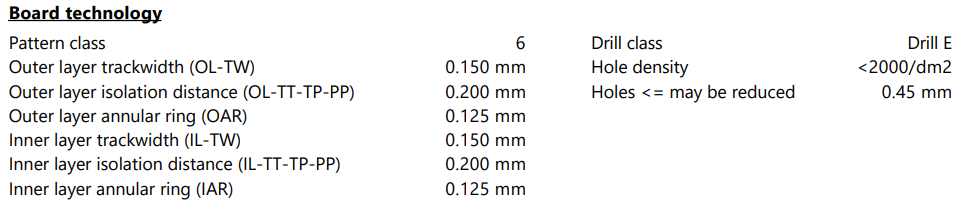
\includegraphics[width=0.9\textwidth]{figures/eurocircuits_report.png}
    \caption{Eurocircuits manufacturing analysis report showing the PCB production classification and drill category.}
    \label{fig:eurocircuits_report}
\end{figure}

\begin{landscape}

    \section{BOM and Costs}

    \small                          % slightly smaller font to fit columns

    \begin{longtable}{
        |c                          % Item
        |p{3cm}                   % Reference
        |c                   % Value
        |p{5cm}                   % MPN
        |l                   % Description
        |c                          % Qty
        |p{1.2cm}                          % Cost 1x
        |p{1.2cm}                          % Cost 10x
        |p{1.2cm}|                         % Cost 100k
    }

        % ---------------------------------------------------------------
        %  CAPTION (shown once at the top of the first page)
        % ---------------------------------------------------------------
        \caption{Bill of Materials with Cost Breakdown}
        \label{tab:bom}\\

        % ---------------------------------------------------------------
        %  HEADER (repeated at the top of every page)
        % ---------------------------------------------------------------
        \hline
        \rowcolor[gray]{0.85}
        \textbf{Item} &
        \textbf{Reference} &
        \textbf{Value} &
        \textbf{MPN} &
        \textbf{Description} &
        \textbf{Qty} &
        \textbf{Cost 1x} &
        \textbf{Cost 10x} &
        \textbf{Cost 100k} \\
        \hline
        \endfirsthead

        \multicolumn{9}{l}{\small\itshape (continued from previous page)}\\[2pt]
        \hline
        \rowcolor[gray]{0.85}
        \textbf{Item} &
        \textbf{Reference} &
        \textbf{Value} &
        \textbf{MPN} &
        \textbf{Description} &
        \textbf{Qty} &
        \textbf{Cost 1x} &
        \textbf{Cost 10x} &
        \textbf{Cost 100k} \\
        \hline
        \endhead

        % ---------------------------------------------------------------
        %  FOOTER (every page except the last)
        % ---------------------------------------------------------------
        \hline
        \multicolumn{9}{r}{\small\itshape (continued on next page)}\\
        \endfoot

        % ---------------------------------------------------------------
        %  LAST FOOTER
        % ---------------------------------------------------------------
        \hline\hline

% ---------------- COMPONENTS ----------------
\multicolumn{5}{|r|}{\textbf{Total for Components}} &
\multicolumn{1}{c|}{ } &
\textbf{28.74\,\euro} &
\textbf{22.18\,\euro} &
\textbf{8.86\,\euro} \\
\hline

% ---------------- PCB ----------------
\multicolumn{5}{|r|}{PCB Manufacturing} &
\multicolumn{1}{c|}{ } &
1.20\,\euro &
1.12\,\euro &
0.16\,\euro \\
\hline

% ---------------- ASSEMBLY BREAKDOWN ----------------
\multicolumn{5}{|r|}{PCB Assembly \textsuperscript{(2)} }&
\multicolumn{1}{c|}{ } &
0.49\,\euro &
0.49\,\euro &
0.33\,\euro  \\
\hline

% ---------------- TOTAL MANUFACTURING ----------------
\multicolumn{5}{|r|}{\textbf{Total for Manufacturing}} &
\multicolumn{1}{c|}{ } &
\textbf{1.69\,\euro} &
\textbf{1.61\,\euro} &
\textbf{0.49\,\euro} \\
\hline

% ---------------- ENCLOSURE ----------------
\multicolumn{5}{|r|}{3D Printed Enclosure \textsuperscript{(2)} } &
\multicolumn{1}{c|}{ } &
0.94\,\euro &
0.94\,\euro &
0.94\,\euro \textsuperscript{(3)}\\
\hline

% ---------------- GRAND TOTAL ----------------
\multicolumn{5}{|r|}{\textbf{Grand Total}} &
\multicolumn{1}{c|}{ } &
\textbf{31.36\,\euro} &
\textbf{24.72\,\euro} &
\textbf{10.29\,\euro} \\
\hline

\endlastfoot

        % ---------------------------------------------------------------
        %  DATA ROWS
        % ---------------------------------------------------------------
        1  & A1 & -- & --
        & PCB Inverted F Antenna 2--4\,GHz & 1
        & -- & -- & -- \\
        \hline

        2  & C1, C2, C3, C6, C7, C11, C16, C20, C22, C23, C25, C28, C29
        & 100\,n & 0603B104K500CT
        & Cap 0.1\,\textmu F, 50\,V, X7R, 10\%, 0603 & 13
        & 0.09\,\euro & 0.02\,\euro & 0.00\,\euro \\
        \hline

        3  & C4, C5, C8 & 10\,\textmu & 0603X106M6R3CT
        & Cap 10\,\textmu F, 6.3\,V, X5R, 20\%, 0603 & 3
        & 0.09\,\euro & 0.03\,\euro & 0.01\,\euro \\
        \hline

        4  & C9, C10, C12 & 12\,p & 0603N120J500CT
        & Cap 12\,pF, 50\,V, C0G NP0, 5\%, 0603 & 3
        & 0.09\,\euro & 0.02\,\euro & 0.00\,\euro \\
        \hline

        5  & C13, C14 & 1.2\,p & CC0603BRNPO9BN1R2
        & Cap 1.2\,pF, 50\,V, C0G NP0, $\pm$0.1\,pF, 0603 & 2
        & 0.09\,\euro & 0.05\,\euro & 0.01\,\euro \\
        \hline

        6  & C15, C24, C27 & 2.2\,\textmu & 0603X225K160CT
        & Cap 2.2\,\textmu F, 16\,V, 10\%, 0603 & 3
        & 0.09\,\euro & 0.03\,\euro & 0.01\,\euro \\
        \hline

        7  & C17, C19 & 470\,n & MCASU168SB5474KTNA01
        & Cap 0.47\,\textmu F, X5R, 10\%, 0603 & 2
        & 0.12\,\euro & 0.07\,\euro & 0.00\,\euro \\
        \hline

        8  & C18 & 4.7\,\textmu & GMC10X5R475K6R3NT
        & Cap 4.7\,\textmu F, 6.3\,V, X5R, 10\%, 0603 & 1
        & 0.09\,\euro & 0.03\,\euro & 0.01\,\euro \\
        \hline

        9  & C21, C26, C32 & 1\,\textmu & 0603B105K250CT
        & Cap 1\,\textmu F, 25\,V, X7R, 10\%, 0603 & 3
        & 0.09\,\euro & 0.02\,\euro & 0.00\,\euro \\
        \hline

        10 & C30 & 4.7\,\textmu & GRM219R6YA475KA73J
        & Cap 4.7\,\textmu F, 35\,V, X5R, 10\%, 0805, 4.8\,m$\Omega$ & 1
        & 0.14\,\euro & 0.08\,\euro & 0.02\,\euro \\
        \hline

        11 & C31 & 47\,\textmu & GRM21BR61A476ME15L
        & Cap 47\,\textmu F, 10\,V, X5R, 20\%, 0805, 0.18\,m$\Omega$ & 1
        & 0.46\,\euro & 0.28\,\euro & 0.11\,\euro \\
        \hline

        12 & IC1 & -- & PAC1951T-1E/4MX
        & IC Current/Voltage Monitor, 1\%, 16\,VQFN & 1
        & 1.00\,\euro & 0.83\,\euro & 0.81\,\euro \\
        \hline

        13 & IC2 & -- & MAX77597ETBB+T
        & 36\,V, 300\,mA Buck Converter, 1.1\,\textmu A $I_q$ & 1
        & 1.65\,\euro & 1.21\,\euro & 0.81\,\euro \\
        \hline

        14 & J1 & -- & MCOT128064N2Z-BM
        & MCOT128064N2Z-BM Display & 1
        & 11.37\,\euro & 10.92\,\euro & 2.11\,\euro \\
        \hline

        15 & J2, J3 & -- & USB4215-03-A
        & USB-C Connector, 5\,A & 2
        & 0.45\,\euro & 0.37\,\euro & 0.23\,\euro \\
        \hline

        16 & J4 & -- & PR20204VBDN
        & Pin Header, 4$\times$2, 2.54\,mm pitch, TH & 1
        & 0.09\,\euro & 0.05\,\euro & 0.03\,\euro \\
        \hline

        17 & L1 & 10\,u & LQM21FN100M80L
        & Ind 10\,\textmu H, 100\,mA, 20\%, 0805 & 1
        & 0.16\,\euro & 0.14\,\euro & 0.07\,\euro \\
        \hline

        18 & L2 & 15\,n & LQG18HN15NJ00D
        & Ind 15\,nH, 600\,mA, 0603, 400\,m$\Omega$ & 1
        & 0.14\,\euro & 0.11\,\euro & 0.06\,\euro \\
        \hline

        19 & L5 & 2.2\,n & LQG18HN2N2S00D
        & Ind 2.2\,nH, 1.1\,A, 0603, 100\,m$\Omega$ & 1
        & 0.14\,\euro & 0.11\,\euro & 0.06\,\euro \\
        \hline

        20 & L6 & 47\,\textmu & ASPI-0615FS-470M-T2
        & Ind 47\,\textmu H, 800\,mA, 370\,m$\Omega$ & 1
        & 0.30\,\euro & 0.25\,\euro & 0.13\,\euro \\
        \hline

        21 & L7 & 1.5\,k & BLM18HE152SN1D
        & Ferrite Bead 1.5\,k$\Omega$, 500\,mA, 0603 & 1
        & 0.19\,\euro & 0.13\,\euro & 0.04\,\euro \\
        \hline

        22 & MH1, MH2, MH3 & -- & --
        & M2 Mounting Hole & 3
        & -- & -- & -- \\
        \hline

        23 & Q1 & -- & SI2365EDS-T1-BE3
        & MOSFET SOT-23 P-Ch, 20\,V, 4.5\,A & 1
        & 0.40\,\euro & 0.24\,\euro & 0.06\,\euro \\
        \hline

        24 & RT1 & -- & 103AP-2
        & NTC Thermistor, 10\,k$\Omega$, 0.5\% & 1
        & 0.60\,\euro & 0.50\,\euro & 0.33\,\euro \\
        \hline

        25 & R1, R6, R7, R8, R16 & 10\,k & WR06X103 JTL
        & Res 10\,k$\Omega$, 0603, 5\%, 0.1\,W & 5
        & 0.09\,\euro & 0.01\,\euro & 0.00\,\euro \\
        \hline

        26 & R2, R13, R18, R19 & 100\,k & WR06X104 JTL
        & Res 100\,k$\Omega$, 0603, 5\%, 0.1\,W & 4
        & 0.09\,\euro & 0.01\,\euro & 0.00\,\euro \\
        \hline

        27 & R3, R4, R14 & 1\,k & WR06X102 JTL
        & Res 1\,k$\Omega$, 0603, 5\%, 0.1\,W & 3
        & 0.09\,\euro & 0.01\,\euro & 0.00\,\euro \\
        \hline

        28 & R5, R9 & 0\,$\Omega$ & WR06X000 PTL
        & Res 0\,$\Omega$, 0603 & 2
        & 0.09\,\euro & 0.01\,\euro & 0.00\,\euro \\
        \hline

        29 & R10 & 10\,m & LVK12R010CER
        & Res 10\,m$\Omega$, 1206, 0.25\%, 0.5\,W & 1
        & 1.31\,\euro & 0.86\,\euro & 0.34\,\euro \\
        \hline

        30 & R11, R12 & 32.4\,$\Omega$ & RMCF0603FT32R4
        & Res 32.4\,$\Omega$, 0603, 1\%, 0.1\,W & 2
        & 0.09\,\euro & 0.02\,\euro & 0.00\,\euro \\
        \hline

        31 & R15 & 5.76\,k & ERA3AEB5761V
        & Res 5.76\,k$\Omega$, 0603, 0.1\%, 0.1\,W & 1
        & 0.09\,\euro & 0.05\,\euro & 0.03\,\euro \\
        \hline

        32 & R17 & 402\,k & RMCF0603FT402K
        & Res 402\,k$\Omega$, 0603, 1\%, 0.1\,W & 1
        & 0.09\,\euro & 0.02\,\euro & 0.00\,\euro \\
        \hline

        33 & R20 & 240\,k & MCR03ERTJ244
        & Res 240\,k$\Omega$, 0603, 5\%, 0.1\,W & 1
        & 0.10\,\euro & 0.01\,\euro & 0.00\,\euro \\
        \hline

        34 & S1 & -- & TS11-674-43-BK-260-RA-D
        & SPST Tactile Switch, TH & 1
        & 0.14\,\euro & 0.12\,\euro & 0.08\,\euro \\
        \hline

        35 & S2 & -- & TL3305CF260QG
        & SPST Tactile Switch, SMD & 1
        & 0.18\,\euro & 0.15\,\euro & 0.09\,\euro \\
        \hline

        36 & TP1--TP7 & -- & --
        & Test Point & 7
        & -- & -- & -- \\
        \hline

        37 & U1 & -- & CC2640R2FRHBR
        & IC RF TxRx + MCU Bluetooth, 32-VFQFN & 1
        & 3.92\,\euro & 3.39\,\euro & 2.47\,\euro \\
        \hline

        38 & Y1 & -- & TSX-3225240000MF15X-AC3
        & Crystal 24\,MHz, 9\,pF, 10\,ppm & 1
        & 0.71\,\euro & 0.61\,\euro & 0.44\,\euro \\
        \hline

        39 & Y2 & -- & FC-135R 32.7680KA-AG0
        & Crystal 32.768\,kHz, 7\,pF, 20\,ppm & 1
        & 0.46\,\euro & 0.40\,\euro & 0.27\,\euro \\

    \end{longtable}

\vspace{0.2cm}
\noindent\footnotesize
\textit{1:} IVA is not included in the calculated costs.\\
\textit{2:} Values are estimated by cost calculator tools provided JLCPCB Manufacturer.\\
\textit{3:} For large-scale production, injection molding is preferred over 3D printing for the plastic cover.


\end{landscape}